%!TEX root = report.tex
\subsection{Journey Planner Bus Timetables}
The Journey Planner Bus Timetables \cite{open_data_feeds_description} contains information on official bus schedules including stops, routes, departures times, departure frequencies, operational notes, as well as the days on which the services run.

The timetables uses the \acrfull{xml} \cite{xml} format, with the schema defined in \gls{transxchange} \cite{transxchange}, the UK nationwide standard for exchanging bus schedules and related data. For this project, we used the General schema version 2.1\cite{transxchange_downloads_and_schema}\cite{transxchange_schema_2.1_xsd}, the latest available version for download. Each \acrshort{xml} file contains the bus timetables for one route. Figure \ref{fig:xml_components} shows the overview of a timetable \acrshort{xml} file.

\begin{figure}
\centering
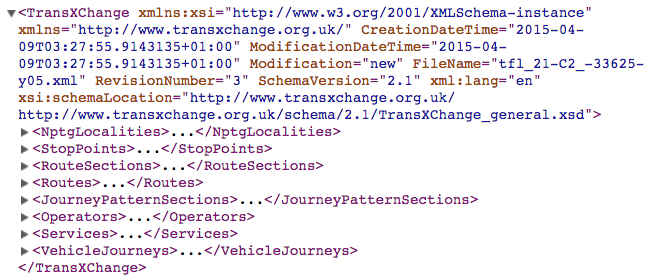
\includegraphics[width=1\textwidth]{figures/xml_components.png}
\caption{\label{fig:xml_components} TfL Journey Planner Timetables Sample XML Overview}
\end{figure}

\subsubsection{Data Structure}
The \gls{transxchange} timetable model has the following seven basic concepts\cite{transxchange_schema_guide}:

\begin{enumerate}
  \item \texttt{Service} contains one or more \texttt{JourneyPattern} elements and one or more \texttt{VehicleJourney} elements. This is the basic concept that brings together the information about a registered bus service.
  \item \texttt{Registration} specifies the registration details for a service.
  \item \texttt{Operator} indicates the entity who runs the service.
  \item \texttt{Route} describes the physical path taken by buses on the service as an ordered list of \texttt{StopPoints}.
  \item \texttt{StopPoint} contains reusable declarations of the stops used by the routes and journey patterns of the schedule. All StopPointRef instances elsewhere in a document are resolved against the contents of the StopPoints element. All stops are defined as being \gls{naptan} points.
  \item \texttt{JourneyPattern} specifies an ordered list of links between the \texttt{StopPoints}, giving the \emph{relative travel times} between each pair of neighbouring stops.
  \item \texttt{VehicleJourney} specifies the individual scheduled journey \emph{at a specific absolute time}.
\end{enumerate}

These elements give a complete official bus schedule for each route with the departure time for each bus journey, the relative bus travel time between stops, and the days on which the service operates on. We extracted the official bus timetables from these \acrshort{xml} files, as discussed in Section \ref{sec: official_tfl_timetable}.
